%%%%%%%%%%%%%%%%%%%%%%%%%%%%%%%%%%%%%%%%%%%%%%%%%%%%%%%%%%%%%%%%%%%%%%%%%%%%%%%%
%2345678901234567890123456789012345678901234567890123456789012345678901234567890
%        1         2         3         4         5         6         7         8

\documentclass[letterpaper, 10 pt, conference]{ieeeconf}  % Comment this line out
                                                          % if you need a4paper
%\documentclass[a4paper, 10pt, conference]{ieeeconf}      % Use this line for a4
                                                          % paper

\IEEEoverridecommandlockouts                              % This command is only
                                                          % needed if you want to
                                                          % use the \thanks command
\overrideIEEEmargins
% See the \addtolength command later in the file to balance the column lengths
% on the last page of the document



% The following packages can be found on http:\\www.ctan.org
\usepackage{graphics} % for pdf, bitmapped graphics files
\usepackage{epsfig} % for postscript graphics files
\usepackage{mathptmx} % assumes new font selection scheme installed
\usepackage{times} % assumes new font selection scheme installed
\usepackage{amsmath} % assumes amsmath package installed
\usepackage{amssymb}  % assumes amsmath package installed
\usepackage{color}

\title{\LARGE \bf
  Titel
}

%\author{ \parbox{3 in}{\centering Huibert Kwakernaak*
%         \thanks{*Use the $\backslash$thanks command to put information here}\\
%         Faculty of Electrical Engineering, Mathematics and Computer Science\\
%         University of Twente\\
%         7500 AE Enschede, The Netherlands\\
%         {\tt\small h.kwakernaak@autsubmit.com}}
%         \hspace*{ 0.5 in}
%         \parbox{3 in}{ \centering Pradeep Misra**
%         \thanks{**The footnote marks may be inserted manually}\\
%        Department of Electrical Engineering \\
%         Wright State University\\
%         Dayton, OH 45435, USA\\
%         {\tt\small pmisra@cs.wright.edu}}
%}

\author{Arthur Boetes, Bruno Eijsvoogel, Robert Hauer, Geert Kapteijns
}

\begin{document}


\maketitle
\thispagestyle{empty}
\pagestyle{empty}


%%%%%%%%%%%%%%%%%%%%%%%%%%%%%%%%%%%%%%%%%%%%%%%%%%%%%%%%%%%%%%%%%%%%%%%%%%%%%%%%
\begin{abstract}

Lorem ipsum dolor sit amet, consectetur adipisicing elit, sed do eiusmod tempor
incididunt ut labore et dolore magna aliqua. Ut enim ad minim veniam, quis
nostrud exercitation ullamco laboris nisi ut aliquip ex ea commodo consequat.
Duis aute irure dolor in reprehenderit in voluptate velit esse cillum dolore eu
fugiat nulla pariatur. Excepteur sint occaecat cupidatat non proident, sunt in
culpa qui officia deserunt mollit anim id est laborum.
\end{abstract}


%%%%%%%%%%%%%%%%%%%%%%%%%%%%%%%%%%%%%%%%%%%%%%%%%%%%%%%%%%%%%%%%%%%%%%%%%%%%%%%%
\section{One-dimensional charge density waves}

Materials in which the electron density $\rho(x)$ is modulated with a wave of
wavelength $\lambda = \frac{2\pi}{Q}$ are said to contain a charge density wave.
In this paper, we will treat a simple model for a one-dimensional chain of atoms containing such a charge density wave:

\begin{align}
H = -t \sum_x (c_x^{\dagger}c_{x+a} + c_x^{\dagger}c_{x-a}) + \sum_x (\mu + \Delta \cos(Qx + \phi))c_x^{\dagger}c_x
\end{align}

The first term describes hopping between sites, and the second term contains the chemical potential and the charge density wave. From the fact that at a band gap opens at $\mu$, it follows that $\mu = -2t\cos(\frac{Qa}{2})$.

If $\lambda = n a$ with $n$ integer and $a$ the lattice spacing, the charge order is said to be commensurate, i.e. the charge modulation is neatly periodic in $n$ lattice sites. Otherwise, the charge order is called incommensurate.

After imposing periodic boundary conditions, commensurate charge order is the only option, and the total amount of lattice sites $N$ must equal a multiple of $\lambda$.

To diagonalize $H$, we first apply the canonical Fourier transform:

$$c_x = \frac{1}{\sqrt{N}}\sum_{0 \leq k < \frac{2\pi}{a}}e^{ikx}c_k$$

The hopping term and the chemical potential both give contributions diagonal in $k$. After writing $\cos(Qx + \phi) = \frac{1}{2}(e^{i(Qx + \phi)} + e^{-i(Qx + \phi)}) $, we see that the charge wave in real space gives an off-diagonal contribution in $k$. The resulting Hamiltonian in Fourier space is:

$$ H = \sum_{0 \leq k < \frac{2\pi}{a}} (\frac{1}{2}\epsilon_k c_k^{\dagger}c_k + \Delta_\phi c_k^{\dagger}c_{k+Q} + \text{H.c.}) $$

Where $\epsilon_k = -2t \cos(ka) + \mu $ and $\Delta_\phi = \Delta e^{i\phi}$, i.e. $\Delta$ acquires a phase corresponding to the offset of the charge distribution.






\subsection{Matrix Form Hamiltonian}
We will take a few steps to put this Hamiltonian in Matrix form.
This will prove to be a more convinient way to perform numerical calculations.\\
First we group terms in the sum over $k$ into $q$ sums over $m$.

\begin{align*}
H &= \sum_{0 \leq k < \frac{2\pi}{a}} (\frac{1}{2}\epsilon_k c_k^{\dagger}c_k + \Delta_\phi c_k^{\dagger}c_{k+Q} + \text{H.c.})\\
&=\sum_{0 \leq k < \frac{2\pi}{qa}} \sum_{m=0}^{q-1}  (\frac{1}{2}\epsilon_{k+\frac{2\pi m}{qa}} c_{k+\frac{2\pi m}{qa}}^{\dagger}c_{k+\frac{2\pi m}{qa}} + \Delta_\phi c_{k+\frac{2\pi m}{qa}}^{\dagger}c_{k+\frac{2\pi m}{qa}+Q} + \text{H.c.})\\
\end{align*}

Since our case is commensurate, we can express $Q=\frac{2\pi}{qa}$. Furthermore we can shift the sum over $m$ by 1,
since $k$ and $k+\frac{2\pi}{a}$ are equivalent points in $k$-space.

\begin{align*}
  &=\sum_{0 \leq k < Q} \sum_{p=1}^{q}  (\frac{1}{2}\epsilon_{k+Qm} c_{k+Qm}^{\dagger}c_{k+Qm} + \Delta_\phi c_{k+Qm}^{\dagger}c_{k+Q(m+1)} + \text{H.c.})\\
  &=\sum_{0\leq k < Q} (c_{k+Q}^{\dagger},c_{k+2Q}^{\dagger},\dots,c_{k+qQ}^{\dagger})\tilde{H}_{k} (c_{k+Q},c_{k+2Q},\dots,c_{k+qQ})^{T} \\
\end{align*}

\begin{align}
\tilde{H}_{k}=\begin{bmatrix}
\epsilon_{k+Q}       & \Delta_\phi     & 0      & \hdots     & 0     & \Delta_\phi^*  \\
\Delta_\phi^*    & \epsilon_{k+2Q} & \Delta_\phi & 0 & \hdots     & 0 \\
0               & \Delta_\phi^* & \ddots & \ddots  &  &\vdots \\
\vdots   & 0 & \ddots &  &  &  0  \\
0 &  \vdots    &  &  &  & \Delta_{\phi} \\
\Delta_\phi & 0 &    \hdots          &0   & \Delta_{\phi}^{*}      & \epsilon_{k+qQ}
\end{bmatrix}
\end{align}




\section{Chern numbers and Electron transport}

Varying the phase of the CDW, does not necessarily transport the electrons along the chain.
The transport depends on the chemical potential.
For $\mu(Q=\frac{ap}{q}) = 0$, we have \textit{no} electron transport.
This corresponds to our Chern numbers being $0$.
This is in agreement with the calculations of section \textbf{???}.
The important connection to make is that the Chern numbers are antisymmetric at the same point as the chemical potential is.
This is the point for which the electron transport changes directions.
The antisymmetry of the Chern numbers is easily seen in the antisymmetry around $\frac{1}{2}$ of the colouring of the spectrum as a function of $\frac{p}{q}$ ie the Hofstadter Butterfly figure \textbf{???}.\\
The transport of electrons along the chain is analogous to the transport of electrons in the integer quantum Hall effect.
In the next subsection we look more carefully at this comparison.

\subsection{The Hofstadter Hamiltonian vs CDW}
Now we will compare our real-space Hamiltonian to that of the tight-binding model on an
isotropic square lattice under a vertical uniform magnetic field in $k$-space \cite{Yoshioka}:
$$
\mathcal{H}=-t\sum_{k_{x},k_{y}}(c_{1}^{\dagger}(\textbf{k}),c_{2}^{\dagger}(\textbf{k}),\dots,c_{q}^{\dagger}(\textbf{k}))\tilde{\mathcal{H}}_{k}(c_{1}(\textbf{k}),c_{2}(\textbf{k}),\dots,c_{q}(\textbf{k}))
$$
$$
\tilde{\mathcal{H}}_{k}=\begin{bmatrix}
E_{k_{y}+2\pi \Phi}      & 1     & 0      & \hdots     & 0     & e^{-iqk_{x}}  \\
1    &E_{k_{y}+4\pi \Phi} & 1 & 0 & \hdots     & 0 \\
0               & 1 & \ddots & \ddots  &  &\vdots \\
\vdots   & 0 & \ddots &  &  &  0  \\
0 &  \vdots    &  &  &  & 1 \\
e^{iqk_{x}} & 0 &    \hdots          &0   & 1      & E_{k_{y}+2\pi q\Phi}
\end{bmatrix}
$$

With $E_{k_{y}+2\pi m\Phi}=2\cos(k_{y}+2\pi m\Phi)$. Where $\Phi$ is in units of the magnetic flux quantum.

This is how to map this situation onto that of the CDW.

\begin{align*}
k_{y} &\leftrightarrow \phi  \\
\Phi &\leftrightarrow \frac{Q}{2\pi} \\
\end{align*}

The $x$-sum in the CDW case goes from sites 1 to $q$.
The length of the chain $q$ is the same as the length of the magnetic unit cells in the lattice.
The phase due to the flux in the lattice case gives us the complex exponential in the corners of our matrix.
Finally to make the mapping work we need to set $\Delta = 2t$ and $a=1$.


\section{Topological classification}

The charge density wave Hamiltonian in $k$-space can be divided in different
classes. Originally the classification was developed for translational or
rotational invariant systems, but because the dihedral group is the only
nontrivial space group another classification is made. When symmetries are taken
into account a topological classification can be made. If a system behaves in
the same way when time is reversed on can say that the system has a time
symmetry. For time symmetry there are 3 options. Either the system is not time
symmetric $(T=0)$, or it is time symmetric $(T^2=1)$ or the system is time
anti-symmetric  $(T^2=-1)$.  Another symmetry  is charge conjugation C. When
this is observed as particle-hole symmetry one can distinguish an occupation of
the hole or an empty hole. When there is a symmetry the  charge conjugation can
be plus $(C^2=1)$ or minus $(C^2=-1)$ and when there is no symmetry  the charge
conjugation number  is zero $(C=0)$.  Because both the time reversal operator T
and the charge conjugation number C are topological invariant their
multiplication $S=T * C $ is also a topological invariant. As a first guess one
would find $3 * 3 = 9 $ topological invariant sectors. But when there is no time
reversal $(T=0)$ and no charge conjugation $(C=0)$, S can have two values. When
a system is symmetric in the combination of time and particle hole symmetry S is
given the value of $1$. When it is not symmetric in the combination of them the
value is $0$. All together there are than $10$ different topological sectors
where S is an invariant. This Tenfold Way classifies the allowed topologies of
all gapped, disordeblack, quadratic fermion theories into ten classes based on the
dimension of the parameter space, see ???. The advantage of this classification is that
these sectors have edge states which are classified by a nonzero Chern number.
Because these edge states do not
depend on small perturbations in the bulk of the material it is possible to
measure variables at the edge that give information of the whole material.
To classify our Hamiltonian we see that there are no zero's on the diagonal,
which exclude the 3 chiral cases. Because the Hamiltonian can be expressed as a 2$\times$2
 matrix, exept in the case of half filling, the four Bogoliubov-de Gennes cases. From the three
 clases left, it must be the one where the Hamiltonian in $k$ space is complex.
 With this reasoning our Hamiltonian fall into the symmetry-free class.


\subsection{Figures and Tables}

Positioning Figures and Tables: Place figures and tables at the top and bottom of columns. Avoid placing them in the middle of columns. Large figures and tables may span across both columns. Figure captions should be below the figures; table heads should appear above the tables. Insert figures and tables after they are cited in the text. Use the abbreviation ÒFig. 1Ó, even at the beginning of a sentence.

\definecolor{black}{rgb}{0.0,0.0,0.0}
\newcommand\T{\rule{0pt}{1em}}

$$
\begin{array}{c|rrr|cccccccc}
\hline
\color{black}{\textrm{class}} & \color{black}{S} & \color{black}{C} & \color{black}{T} & \color{black}{d=0} & \color{black}{1} & \color{black}{2} & \color{black}{3} & \color{black}{4} & \color{black}{5} & \color{black}{6} & \color{black}{7}\T\\
\hline \color{black}{\textrm{A}} & \color{black}{} & \color{black}{} & \color{black}{} & \color{black}{\mathbb{Z}} & \color{black}{} & \color{black}{\mathbb{Z}} & \color{black}{} & \color{black}{\mathbb{Z}} & \color{black}{} & \color{black}{\mathbb{Z}} & \color{black}{}\T\\
\color{black}{\textrm{AIII}} & \color{black}{1} & \color{black}{} & \color{black}{} & \color{black}{} & \color{black}{\mathbb{Z}} & \color{black}{} & \color{black}{\mathbb{Z}} & \color{black}{} & \color{black}{\mathbb{Z}} & \color{black}{} & \color{black}{\mathbb{Z}}\T\\
\hline \color{black}{\textrm{AI}} & \color{black}{} & \color{black}{} & \color{black}{1} & \color{black}{\mathbb{Z}} & \color{black}{} & \color{black}{} & \color{black}{} & \color{black}{2\mathbb{Z}} & \color{black}{} & \color{black}{\mathbb{Z}_2} & \color{black}{\mathbb{Z}_2}\T\\
\color{black}{\textrm{BDI}} & \color{black}{1} & \color{black}{1} & \color{black}{1} & \color{black}{\mathbb{Z}_2} & \color{black}{\mathbb{Z}} & \color{black}{} & \color{black}{} & \color{black}{} & \color{black}{2\mathbb{Z}} & \color{black}{} & \color{black}{\mathbb{Z}_2}\T\\
\color{black}{\textrm{D}} & \color{black}{} & \color{black}{1} & \color{black}{} & \color{black}{\mathbb{Z}_2} & \color{black}{\mathbb{Z}_2} & \color{black}{\mathbb{Z}} & \color{black}{} & \color{black}{} & \color{black}{} & \color{black}{2\mathbb{Z}} & \color{black}{}\T\\
\color{black}{\textrm{DIII}} & \color{black}{1} & \color{black}{1} & \color{black}{-1} & \color{black}{} & \color{black}{\mathbb{Z}_2} & \color{black}{\mathbb{Z}_2} & \color{black}{\mathbb{Z}} & \color{black}{} & \color{black}{} & \color{black}{} & \color{black}{2\mathbb{Z}}\T\\
\color{black}{\textrm{AII}} & \color{black}{} & \color{black}{} & \color{black}{-1} & \color{black}{2\mathbb{Z}} & \color{black}{} & \color{black}{\mathbb{Z}_2} & \color{black}{\mathbb{Z}_2} & \color{black}{\mathbb{Z}} & \color{black}{} & \color{black}{} & \color{black}{}\T\\
\color{black}{\textrm{CII}} & \color{black}{1} & \color{black}{-1} & \color{black}{-1} & \color{black}{} & \color{black}{2\mathbb{Z}} & \color{black}{} & \color{black}{\mathbb{Z}_2} & \color{black}{\mathbb{Z}_2} & \color{black}{\mathbb{Z}} & \color{black}{} & \color{black}{}\T\\
\color{black}{\textrm{C}} & \color{black}{} & \color{black}{-1} & \color{black}{} & \color{black}{} & \color{black}{} & \color{black}{2\mathbb{Z}} & \color{black}{} & \color{black}{\mathbb{Z}_2} & \color{black}{\mathbb{Z}_2} & \color{black}{\mathbb{Z}} & \color{black}{}\T\\
\color{black}{\textrm{CI}} & \color{black}{1} & \color{black}{-1} & \color{black}{1} & \color{black}{} & \color{black}{} & \color{black}{} & \color{black}{2\mathbb{Z}} & \color{black}{} & \color{black}{\mathbb{Z}_2} & \color{black}{\mathbb{Z}_2} & \color{black}{\mathbb{Z}}\\
\hline
\end{array}
$$
%    \begin{figure}[thpb]
%       \centering
%       \framebox{\parbox{3in}{We suggest that you use a text box to insert a graphic (which is ideally a 300 dpi TIFF or EPS file, with all fonts embedded) because, in an document, this method is somewhat more stable than directly inserting a picture.
% }}
%       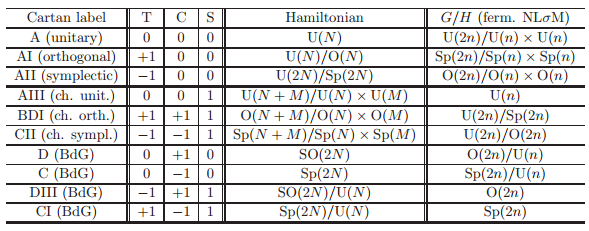
\includegraphics[scale=.5]{ten_fold_way.png}
%       \caption{Inductance of oscillation winding on amorphous
%        magnetic core versus DC bias magnetic field}
%       \label{figurelabel}
%    \end{figure}


Figure Labels: Use 8 point Times New Roman for Figure labels. Use words rather than symbols or abbreviations when writing Figure axis labels to avoid confusing the reader. As an example, write the quantity ÒMagnetizationÓ, or ÒMagnetization, MÓ, not just ÒMÓ. If including units in the label, present them within parentheses. Do not label axes only with units. In the example, write ÒMagnetization (A/m)Ó or ÒMagnetization {A[m(1)]}Ó, not just ÒA/mÓ. Do not label axes with a ratio of quantities and units. For example, write ÒTemperature (K)Ó, not ÒTemperature/K.Ó

\section{CONCLUSIONS}

A conclusion section is not requiblack. Although a conclusion may review the main points of the paper, do not replicate the abstract as the conclusion. A conclusion might elaborate on the importance of the work or suggest applications and extensions.

\addtolength{\textheight}{-12cm}   % This command serves to balance the column lengths
                                  % on the last page of the document manually. It shortens
                                  % the textheight of the last page by a suitable amount.
                                  % This command does not take effect until the next page
                                  % so it should come on the page before the last. Make
                                  % sure that you do not shorten the textheight too much.


\bibliographystyle{plain}
\bibliography{references}


\end{document}
